\documentclass[12pt]{article}

% Language and encoding
\usepackage[utf8]{inputenc}
\usepackage[T1]{fontenc}
\usepackage[english]{babel}

% Math and fonts
\usepackage{amsmath, amsfonts}

% Layout
\usepackage{geometry}
\geometry{a4paper, margin=2.5cm}
\usepackage{setspace}
\usepackage{indentfirst}
\usepackage{graphicx}
\usepackage{booktabs}
\usepackage{caption}
\usepackage{pgfplots}
\pgfplotsset{compat=1.17}
\usepackage{tikz}
\usetikzlibrary{shapes.geometric, arrows.meta, positioning}

% Title
\title{Quantization Strategies for Low-Resource Hardware in Deep Learning Applications}
\author{Caio Martins de Abreu}
\date{}

\begin{document}

\maketitle

\begin{abstract}
This work investigates quantization techniques applied to computational systems with limited hardware resources, focusing on machine learning and signal processing applications. Quantization allows for the representation of numerical data with reduced precision, significantly decreasing memory usage and computational cost. Such techniques are essential for embedded and energy-constrained devices. This study explores and evaluates different quantization strategies to balance accuracy, efficiency, and hardware compatibility.
\end{abstract}

\section{Introduction}

The exponential growth of deep neural network (DNN) applications, especially in computer vision, has increased the demand for deploying such models on embedded platforms like Field-Programmable Gate Arrays (FPGAs). Although FPGAs offer high performance and flexibility, implementing full-precision models (e.g., 32-bit floating-point) on these platforms is often inefficient in terms of power consumption, logic utilization, and memory bandwidth.

In this context, post-training quantization (PTQ) has emerged as a promising solution to reduce model complexity without requiring retraining. Among the PTQ techniques, methods like Accurate and Hardware-Compatible Post-Training Quantization (AHCPTQ) have shown the ability to preserve model accuracy while enabling compatibility with hardware-optimized arithmetic, which is critical for FPGA-based implementations.

Additionally, trainable fixed-point quantization approaches, such as those proposed by Lin et al., demonstrate that integrating quantization into the training process can enhance computational efficiency without degrading predictive performance. This strategy leverages FPGA flexibility in defining data paths and word lengths to create hardware-aware models.

Furthermore, replacing standard floating-point formats with reduced-precision representations — such as half-precision (16-bit) or custom floating-point types — has also been explored to improve throughput and energy efficiency in FPGA-based accelerators.

This work proposes the evaluation and implementation of quantization techniques on convolutional neural networks, focusing on strategies that balance accuracy, computational efficiency, and hardware compatibility. The goal is to enable efficient inference in real-world embedded AI scenarios.

\section{Methodology}

This study adopts an experimental approach to evaluate the impact of post-training quantization techniques on convolutional neural networks (CNNs) targeting embedded hardware. Two widely used vision models were selected for analysis: the \textit{Segment Anything Model} (SAM) by Meta AI, and \textit{You Only Look Once} (YOLO). The focus was on preserving predictive quality after quantization for deployment in resource-constrained environments.

\subsection{Selected Models}

SAM was selected for its versatility in image segmentation, while YOLO represents a well-established solution for real-time object detection. These models serve as representative benchmarks for assessing the behavior of quantization across distinct vision tasks.

\subsection{Quantization Techniques}

Post-training quantization (PTQ) was applied using native tools from the PyTorch framework, without altering model architectures.

\begin{enumerate}
    \item \textit{Dynamic quantization (SAM):} applied to weights using 8-bit integers (INT8), while activations remain in floating point. Quantization occurs at inference time and requires no calibration.
    
    \item \textit{Static quantization (YOLO):} applied to both weights and activations, using a calibration dataset to determine optimal quantization ranges. This approach offers greater efficiency gains but may impact accuracy more significantly.
\end{enumerate}

\subsection{Experimental Procedure}

Quantization was performed directly on pre-trained models using PyTorch 2.6. All experiments were conducted in a controlled software environment, emulating conditions similar to those found in embedded hardware platforms.

\subsection{Evaluation Criteria}

A qualitative evaluation was conducted based on the following criteria:

\begin{enumerate}
    \item Visual quality of the outputs (segmentation masks from SAM and detection boxes from YOLO);
    \item Semantic coherence between input and prediction;
    \item Structural consistency compared to the original full-precision models.
\end{enumerate}

Although no formal quantitative metrics (e.g., IoU or mAP) were applied, the qualitative assessment provided sufficient insight into the practical impact of quantization on perceptual performance and deployment feasibility.

\subsection{Tools}

All experiments were carried out using PyTorch 2.6, leveraging its built-in quantization features. The models were kept intact to ensure compatibility with export formats such as ONNX, facilitating future integration with FPGA synthesis flows.

\section{Quantization Workflow}

\begin{figure}[h]
\centering
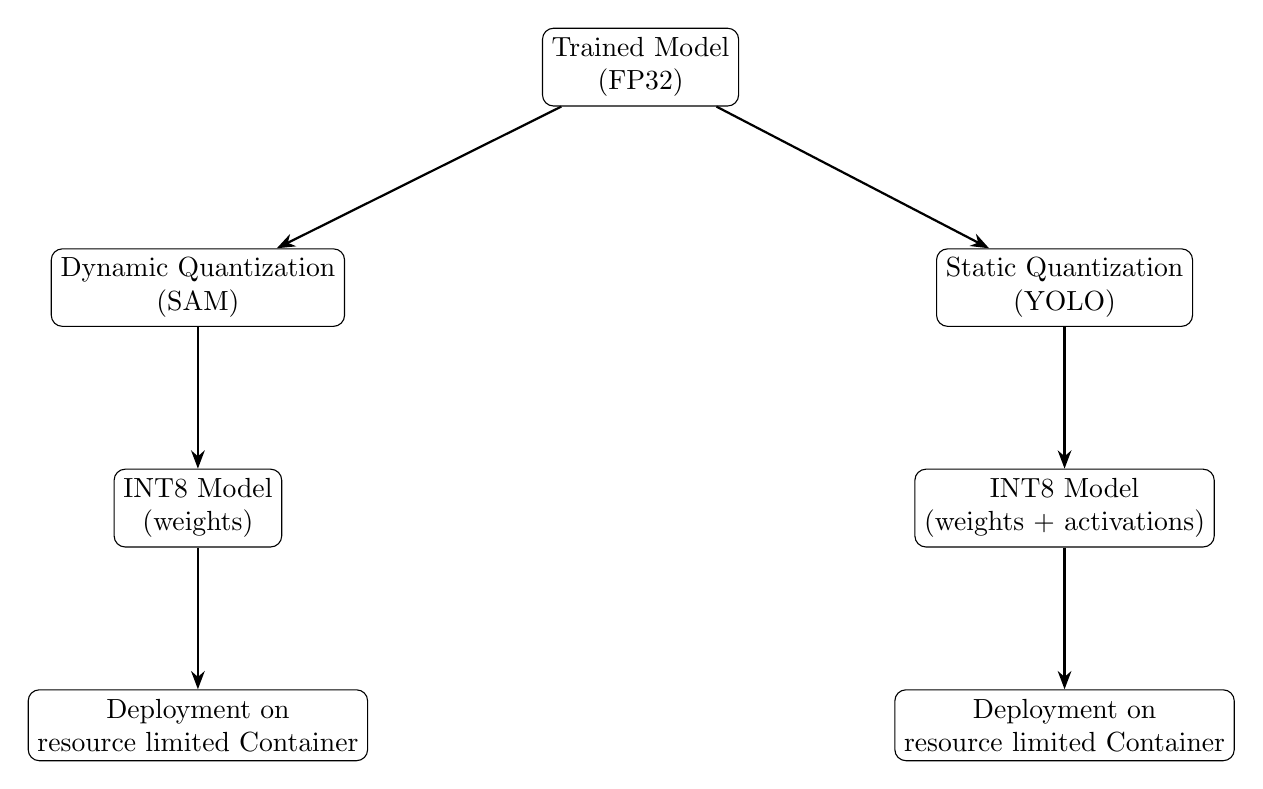
\begin{tikzpicture}[node distance=1.8cm and 2.5cm]
  \tikzstyle{block} = [rectangle, rounded corners, draw, align=center, minimum height=2.5em]
  \tikzstyle{arrow} = [thick, ->, >=Stealth]

  \node[block] (model) {Trained Model\\(FP32)};
  \node[block, below left=of model] (dyn) {Dynamic Quantization\\(SAM)};
  \node[block, below right=of model] (stat) {Static Quantization\\(YOLO)};
  \node[block, below=of dyn] (infd) {INT8 Model\\(weights)};
  \node[block, below=of stat] (infs) {INT8 Model\\(weights + activations)};
  \node[block, below=of infd] (hw1) {Deployment on \\ resource limited Container};
  \node[block, below=of infs] (hw2) {Deployment on \\ resource limited Container};

  \draw[arrow] (model) -- (dyn);
  \draw[arrow] (model) -- (stat);
  \draw[arrow] (dyn) -- (infd);
  \draw[arrow] (stat) -- (infs);
  \draw[arrow] (infd) -- (hw1);
  \draw[arrow] (infs) -- (hw2);
\end{tikzpicture}
\caption{Quantization workflow for SAM and YOLO using PyTorch}
\label{fig:quantization-flow}
\end{figure}

\section{Results Overview}

\begin{table}[h]
\centering
\caption{Qualitative comparison before and after quantization}
\label{tab:comparison}
\begin{tabular}{@{}lccc@{}}
\toprule
\textbf{Model} & \textbf{Precision} & \textbf{Inference Speed} & \textbf{Visual Quality} \\
\midrule
SAM (Original) & FP32   & Low     & High \\
SAM (Quantized) & INT8 (weights) & Moderate & High \\
YOLO (Original) & FP32   & Moderate  & High \\
YOLO (Quantized) & INT8 (weights + activations) & High & Slightly reduced \\
\bottomrule
\end{tabular}
\end{table}

\end{document}